\documentclass{article}
\usepackage[utf8]{vietnam} 
\usepackage[most]{tcolorbox} 
\usepackage{listings} 
\usepackage{xcolor} 
\usepackage{graphicx} % Gói bắt buộc để chèn hình ảnh
\usepackage{amsmath}  % Gói hỗ trợ gõ toán học cao cấp
% 1. GÓI ĐỊNH DẠNG LỀ TRANG GIẤY (Căn lề 2cm đều bốn cạnh)
\usepackage[top=2cm, bottom=2cm, left=2cm, right=2cm]{geometry}
\usepackage{enumitem}
\usepackage[most]{tcolorbox}

% --- KHAI BÁO GÓI VẼ HÌNH TIKZ ---
\usepackage{tikz}
\usetikzlibrary{calc} % Thư viện bổ trợ tính toán tọa độ nâng cao

\tcbuselibrary{skins, listings}

% Bảng màu Dark Mode cao cấp (Phong cách Dracula/Material)
\definecolor{codebg}{HTML}{1E1E2E}      
\definecolor{codeframe}{HTML}{313244}   
\definecolor{codekey}{HTML}{F38BA8}     
\definecolor{codestring}{HTML}{A6E3A1}  
\definecolor{codenumber}{HTML}{585B70}  
\definecolor{noteframe}{HTML}{89B4FA}   
\definecolor{notebg}{HTML}{F3F8FF}      

% --- BỔ SUNG ĐOẠN ĐỊNH NGHĨA NGÔN NGỮ JSON CHO LISTINGS (Đặt trước \newtcblisting) ---
\lstdefinelanguage{json}{
  string=[b]",
  stringstyle=\color{codestring},
  keywordstyle=\color{codekey},
  commentstyle=\color{gray},
}

% Cấu hình khối hiển thị Code chuyên nghiệp
\newtcblisting{customjson}{
  arc=5mm,                    
  boxrule=1pt,                
  colback=codebg,             
  colframe=codeframe,         
  enhanced,
  drop shadow={black!20!white}, 
  title=\textbf{📄 settings.json}, 
  coltitle=white,
  attach boxed title to top left={yshift=-2mm, xshift=5mm},
  % Thay rounded corners thành kiểu gán góc cụ thể để tương thích 100%
  boxed title style={colback=codeframe, sharp corners, rounded corners=north}, 
  listing only,
  listing options={
    language=json,             
    basicstyle=\small\ttfamily\color{white},
    xleftmargin=0.6cm,        
    showstringspaces=false,
    tabsize=1
  }
}

% Cấu hình hộp ghi chú
\newtcolorbox{ghichu}{
  enhanced,
  colback=notebg, 
  colframe=noteframe, 
  boxrule=0pt,                    % Ẩn các viền khác để tạo nét phẳng tối giản
  leftrule=4pt,                   % Tạo vạch màu dày chính xác 4pt ở riêng lề trái
  sharp corners,                  
  title=\textbf{💡 Ghi nhớ quan trọng},
  coltitle=noteframe!50!black,
  attach boxed title to top left={yshift=-2mm, xshift=2mm},
  boxed title style={colback=notebg, boxrule=0pt}
}

\title{\textbf{Cẩm Nang Tự Học LaTeX Cơ Bản}}
\author{\textbf{Lê Quốc Hải}}
\date{\today}

\begin{document}

\maketitle

% Tự động tạo mục lục siêu đẹp
\tableofcontents
\newpage

\section{Hướng dẫn thiết lập ban đầu}

\subsection{Phân tầng mục}

\begin{enumerate}
    \item Thiết lập môi trường Linux
    \begin{enumerate}
        \item Cài đặt gói TeX Live Full.
        \item Tải cấu hình VS Code.
        \begin{enumerate}
            \item Sửa file \texttt{settings.json}.
        \end{enumerate}
    \end{enumerate}
    \item Bắt đầu soạn thảo.
\end{enumerate}

% Kiểu chữ La Mã viết thường (i, ii, iii)
\begin{enumerate}[label=\roman*)]
    \item Nội dung mục i
    \item Nội dung mục ii
\end{enumerate}

% Kiểu chữ cái viết hoa (A, B, C)
\begin{enumerate}[label=\Alph*.]
    \item Nội dung mục A
    \item Nội dung mục B
\end{enumerate}

\subsection{Phím tắt thông dụng trên VS Code}

\begin{itemize}
    \item \textbf{Ctrl + S}: Lưu file và tự động biên dịch (Save and build).
    \item \textbf{Ctrl + Alt + C}: Xóa sạch các file rác phát sinh (Remove build output).
\end{itemize}

* Hoặc dùng enumerate:

\begin{enumerate}
    \item Bước đầu tiên: Nhấn \textbf{Ctrl + S}.
    \item Bước thứ hai: Kiểm tra file PDF trong thư mục \textit{build}.
    \item Bước cuối cùng: Dọn dẹp file rác bằng \textbf{Ctrl + Alt + C}.
\end{enumerate}

\begin{ghichu}
    Nếu phím tắt \textbf{Ctrl + Alt + C} không hoạt động, hãy kiểm tra xem bạn đã cài đặt công cụ dọn dẹp trong extension \textit{LaTeX Workshop} chưa.
\end{ghichu}

\subsection{Cấu hình hệ thống gọn gàng}
Để gom toàn bộ file rác vào một nơi, hãy thêm đoạn mã sau vào file cấu hình \texttt{settings.json}:

\begin{customjson}
"latex-workshop.latex.autoClean.run": "onFailed",
    // 1. vscode with build/ and preview
    "latex-workshop.latex.outDir": "%DIR%/build",
    // 2. Setting Latexmk workdir config at build/
    "latex-workshop.latex.tools": [
        {
            "name": "latexmk",
            "command": "latexmk",
            "args": [
                "-synctex=1",
                "-interaction=nonstopmode",
                "-file-line-error",
                "-pdf",
                "-f",
                "-outdir=%DIR%/build",
                "%DOC%"
            ]
        }
    ],
    // 3. Declare Recipe to VS Code call above tool
    "latex-workshop.latex.recipes": [
        {
            "name": "latexmk",
            "tools": [
                "latexmk"
            ]
        }
    ],
    "[latex]": {
        "editor.defaultFormatter": "James-Yu.latex-workshop",
        "editor.formatOnSave": false
    },
    "[jsonc]": {
        "editor.defaultFormatter": "vscode.json-language-features",
    }
\end{customjson}

\section{Kỹ năng soạn thảo cốt lõi}

\subsection{Chèn công thức toán học}
LaTeX nổi tiếng nhất nhờ khả năng gõ toán học. Bạn có hai cách trình bày:
\begin{itemize}
    \item \textbf{Toán học nội dòng (Inline):} 
    Nằm ngay trong đoạn văn bằng cách kẹp giữa hai dấu \texttt{\$}. 
    Ví dụ: Phương trình bậc hai có dạng $ax^2 + bx + c = 0$.
    \item \textbf{Toán học hiển thị biệt lập (Display):} 
    Kẹp giữa \texttt{\$\$} hoặc 
    dùng môi trường \texttt{equation} để tự động đánh số thứ tự câu hỏi:
\end{itemize}

\subsection{Tạo bảng dữ liệu (Table)}
Bảng trong LaTeX được quản lý rất chặt chẽ thông qua môi trường \texttt{tabular}. Dưới đây là cấu trúc một bảng cơ bản gọn gàng:

\begin{center}
    \begin{tabular}{|c|l|r|}
        \hline
        \textbf{STT} & \textbf{Tên Phầm Mềm}    & \textbf{Đánh Giá} \\ \hline
        1            & VS Code + LaTeX Workshop & 9.5 / 10          \\ \hline
        2            & TeXstudio thuần túy      & 8.0 / 10          \\ \hline
    \end{tabular}
\end{center}

\subsection{Chèn hình ảnh vào văn bản}
Để chèn hình ảnh, bạn cần bỏ file ảnh (ví dụ: \texttt{logo.png}) vào cùng thư mục chứa code và gọi lệnh sau:

\begin{verbatim}
\begin{figure}[h]
    \centering
    \includegraphics[width=0.5\textwidth]{logo.png}
    \caption{Hình ảnh minh họa cho bài viết}
\end{figure}
\end{verbatim}

\begin{ghichu}
    Tham số \texttt{[h]} (here) có nghĩa là ra lệnh cho LaTeX ưu tiên đặt hình ảnh ngay tại vị trí bạn viết code, tránh bị trôi sang trang khác một cách tự động.
\end{ghichu}

\section{Cẩm nang cú pháp gõ toán học (Math Syntax)}\label{section:toanhoc}


\subsection{Tích phân}
Trong đó:
\begin{itemize}
    \item[$f(x)$:] Hàm số cần tính tích phân (ở đây là hàm phân thức $1/x$).
    \item[$a, b$:] Lần lượt là cận dưới và cận trên của tích phân.
    \item[$\ln$:] Hàm số logarit tự nhiên (cơ số $e$).
\end{itemize}
\begin{equation}
    \label{eq:tichphan}
    f(x) = \int_{a}^{b} \frac{1}{x} \,dx = \ln|b| - \ln|a|
\end{equation}

\subsection{Hệ phương trình và Ma trận (Nâng cao)}
Để gõ hệ phương trình có dấu ngoặc nhọn lớn ở bên trái, ta sử dụng môi trường \texttt{cases}. Đối với ma trận dữ liệu, ta dùng môi trường \texttt{pmatrix} (ngoặc đơn) hoặc \texttt{vmatrix} (định thức):

\begin{equation}
    \begin{cases}
        2x + y - z = 4 \\
        x - 3y + 2z = -1 \\
        3x + 2y + z = 1
    \end{cases}
    \quad \Rightarrow \quad
    A = \begin{pmatrix}
        2 & 1 & -1 \\
        1 & -3 & 2 \\
        3 & 2 & 1
    \end{pmatrix}
\end{equation}

\subsection{Chuỗi phương trình biến đổi dài (Căn chỉnh theo dấu bằng)}
Khi giải toán, nếu phương trình quá dài hoặc cần xuống dòng căn thẳng hàng theo dấu bằng ($=$), tuyệt đối không dùng môi trường \texttt{equation} thông thường mà phải dùng \texttt{align} kết hợp ký tự \texttt{\&}:

\begin{align}
    (x + y)^3 &= (x + y)(x + y)^2 \\
              &= (x + y)(x^2 + 2xy + y^2) \\
              &= x^3 + 3x^2y + 3xy^2 + y^3 \label{eq:hangdangthuc}
\end{align}

\subsection{Bảng tra cứu nhanh ký hiệu toán học phổ biến}
Dưới đây là danh sách tổng hợp các syntax cốt lõi nhất khi soạn thảo tài liệu kỹ thuật:

\begin{itemize}
    \item \textbf{Phân số ($\frac{a}{b}$):} Sử dụng cú pháp \texttt{\textbackslash frac\{tử\}\{mẫu\}}.
    \item \textbf{Căn thức ($\sqrt[n]{x}$):} Căn bậc hai dùng \texttt{\textbackslash sqrt\{x\}}, căn bậc $n$ dùng \texttt{\textbackslash sqrt[n]\{x\}}.
    \item \textbf{Chỉ số trên và dưới ($x_{i}^2$):} Chỉ số dưới (subscript) dùng dấu gạch dưới \texttt{\_}, chỉ số trên (mũ/superscript) dùng dấu mũ \texttt{\^}. Nếu phần chỉ số có nhiều hơn 1 ký tự, bắt buộc phải bao bọc trong cặp dấu ngoặc nhọn \texttt{\{...\}}. Ví dụ: \texttt{x\_\{i+1\}\^{}\{n+2\}}.
    \item \textbf{Tổng và Giới hạn ($\sum$, $\lim$):} Tự động căn lề trên dưới đẹp mắt khi đặt trong khối biệt lập:
\end{itemize}

\begin{equation}
    \lim_{n \to \infty} \sum_{i=1}^{n} \frac{1}{i^2} = \frac{\pi^2}{6}
\end{equation}

\subsection{Ký hiệu Hy Lạp và Toán học tập hợp}
\begin{itemize}
    \item \textbf{Chữ cái Hy Lạp:} Chỉ cần gõ tên chữ cái bằng tiếng Anh kèm dấu gạch chéo ngược. Ví dụ: \texttt{\textbackslash alpha} ($\alpha$), \texttt{\textbackslash beta} ($\beta$), \texttt{\textbackslash pi} ($\pi$), \texttt{\textbackslash Delta} ($\Delta$ - viết hoa chữ cái đầu sẽ cho ra ký hiệu dạng hoa).
    \item \textbf{Quan hệ tập hợp:} Thuộc \texttt{\textbackslash in} ($\in$), không thuộc \texttt{\textbackslash notin} ($\notin$), tập hợp con \texttt{\textbackslash subset} ($\subset$), tương đương \texttt{\textbackslash equiv} ($\equiv$).
\end{itemize}

subsection{Các loại Ma trận (Matrix Syntax)}
Để viết ma trận, bạn bắt buộc phải đặt chúng trong môi trường toán học (như \texttt{equation}). Ký tự \texttt{\&} dùng để chuyển sang cột tiếp theo, và \texttt{\textbackslash\textbackslash} dùng để xuống dòng mới.

\begin{itemize}
    \item \textbf{Ma trận ngoặc đơn (pmatrix):} Thường dùng cho ma trận hệ số tiêu chuẩn.
    \item \textbf{Ma trận ngoặc vuông (bmatrix):} Phong cách viết ma trận phổ biến trong giáo trình Việt Nam.
    \item \textbf{Định thức ma trận (vmatrix):} Thay dấu ngoặc bằng hai vạch thẳng đứng để tính định thức (Determinant).
    \item \textbf{Ma trận dấu chấm lửng (Đại số nâng cao):} Sử dụng các lệnh \texttt{\textbackslash cdots} (chấm ngang), \texttt{\textbackslash vdots} (chấm dọc), và \texttt{\textbackslash ddots} (chấm chéo) để biểu diễn ma trận cấp $n$.
\end{itemize}

\begin{equation}
    \text{pmatrix} = \begin{pmatrix}
        a & b \\
        c & d
    \end{pmatrix}
    \quad
    \text{bmatrix} = \begin{bmatrix}
        1 & 0 & 0 \\
        0 & 1 & 0 \\
        0 & 0 & 1
    \end{bmatrix}
    \quad
    \text{vmatrix} = \begin{vmatrix}
        x_{11} & x_{12} \\
        x_{21} & x_{22}
    \end{vmatrix}
\end{equation}

\subsection{Ma trận tổng quát cấp $n \times n$}
Dưới đây là cú pháp để biểu diễn một ma trận có kích thước vô hạn dùng các đường chấm lửng toán học:

\begin{equation}
    A = \begin{bmatrix}
        a_{11} & a_{12} & \cdots & a_{1n} \\
        a_{21} & a_{22} & \cdots & a_{2n} \\
        \vdots & \vdots & \ddots & \vdots \\
        a_{m1} & a_{m2} & \cdots & a_{mn}
    \end{bmatrix}
\end{equation}

\subsection{Logarit, Lượng giác và Đạo hàm (Syntax)}

\begin{itemize}
    \item \textbf{Hàm Lượng giác:} Luôn sử dụng lệnh \texttt{\textbackslash sin}, \texttt{\textbackslash cos}, \texttt{\textbackslash tan} để chữ đứng thẳng. Ví dụ: $\sin^2(x) + \cos^2(x) = 1$.
    \item \textbf{Hàm Logarit:} Logarit tự nhiên dùng \texttt{\textbackslash ln}, logarit cơ số bất kỳ dùng \texttt{\textbackslash log\_b\{x\}}. Ví dụ: $\log_2(8) = 3$.
    \item \textbf{Đạo hàm:} Bạn có thể viết dấu phẩy đạo hàm $f'(x)$ hoặc dùng định dạng phân số đạo hàm của Leibniz \texttt{\textbackslash frac\{d y\}\{d x\}}.
\end{itemize}

\noindent Dưới đây là ví dụ tổng hợp các công thức kết hợp mở rộng:

\begin{equation}
    \frac{d}{dx}\Big( \ln|x| \Big) = \frac{1}{x} \quad \text{và} \quad \frac{d}{dx}\Big( \sin(x) \Big) = \cos(x)
\end{equation}

\subsection{Đạo hàm cấp cao và Đạo hàm riêng (Nâng cao)}
Nếu bạn cần viết đạo hàm cấp 2 hoặc đạo hàm riêng phần (Partial Derivative) trong các phương trình toán lý, hãy sử dụng ký hiệu \texttt{\textbackslash partial}:

\begin{equation}
    f''(x) = \frac{d^2 f}{dx^2} \qquad \text{và} \qquad \frac{\partial^2 u}{\partial x^2} + \frac{\partial^2 u}{\partial y^2} = 0
\end{equation}

Lệnh \texttt{\textbackslash Big(} và \texttt{\textbackslash Big)}: 
Giúp phóng to kích thước của dấu ngoặc đơn bao bọc bên ngoài cụm 
\texttt{\textbackslash \(\ln\vert{}x\vert{}\)} để nó ôm trọn vẹn ký hiệu trị tuyệt đối, 
tránh dấu ngoặc bị quá lùn so với công thức.
Ký hiệu \texttt{\textbackslash \qquad:} Tương tự như \texttt{\textbackslash \quad} nhưng tạo ra một khoảng trống rộng gấp đôi, 
rất thích hợp để ngăn cách hai vế công thức độc lập trên cùng một dòng.

\section{Vẽ hình bằng gói TikZ}

Dưới đây là một ví dụ minh họa về hình học phẳng (Đường tròn và tam giác nội tiếp) được vẽ trực tiếp bằng mã nguồn LaTeX:

\begin{center}
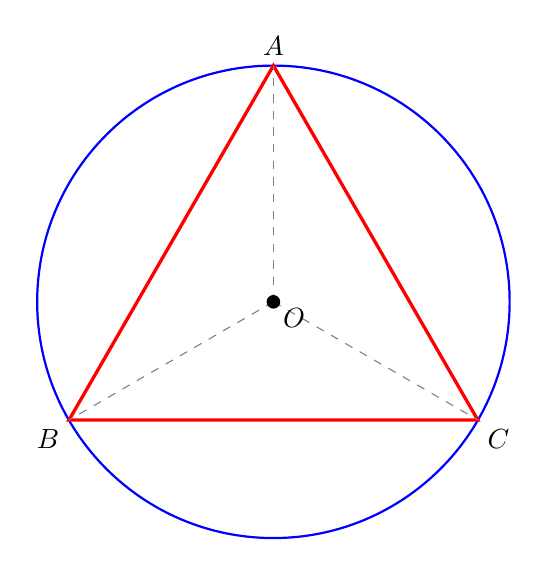
\begin{tikzpicture}[scale=1.5] % scale=1.5 dùng để phóng to hình vẽ lên 1.5 lần

    % 1. Vẽ đường tròn tâm O(0,0), bán kính R = 2cm (màu xanh dương nhạt)
    \draw[blue, thick] (0,0) circle (2cm);
    
    % 2. Xác định tọa độ 3 đỉnh của tam giác
    \coordinate (A) at (0,2);       % Đỉnh A nằm trên đỉnh đường tròn
    \coordinate (B) at (-1.73,-1);  % Đỉnh B góc dưới trái
    \coordinate (C) at (1.73,-1);   % Đỉnh C góc dưới phải
    \coordinate (O) at (0,0);       % Tâm O
    
    % 3. Vẽ các cạnh của tam giác (màu đỏ, nét đậm)
    \draw[red, very thick] (A) -- (B) -- (C) -- cycle;
    
    % 4. Vẽ các đường nét đứt nối từ tâm O đến các đỉnh
    \draw[dashed, gray] (O) -- (A);
    \draw[dashed, gray] (O) -- (B);
    \draw[dashed, gray] (O) -- (C);
    
    % 5. Đánh dấu điểm tâm O bằng một chấm tròn nhỏ
    \filldraw[black] (O) circle (1.5pt);
    
    % 6. Dán nhãn tên các đỉnh (A, B, C, O) vào hình vẽ
    \node[above] at (A) {$A$};
    \node[below left] at (B) {$B$};
    \node[below right] at (C) {$C$};
    \node[right, yshift=-2mm] at (O) {$O$};

\end{tikzpicture}
\end{center}

\section{Giải thích các lệnh TikZ cơ bản}
\begin{itemize}
    \item \texttt{\textbackslash draw[thuộc\_tính] (tọa\_độ\_1) -{}- (tọa\_độ\_2);}: Dùng để vẽ một đoạn thẳng nối liền 2 điểm.
    \item \texttt{circle (bán\_kính);}: Lệnh vẽ đường tròn tại tọa độ đứng trước nó.
    \item \texttt{cycle}: Lệnh ép đường vẽ tự động khép kín về điểm xuất phát đầu tiên (rất tiện khi vẽ đa giác).
    \item \texttt{[dashed]}: Thuộc tính vẽ nét đứt (thường dùng cho đường cao, đường trung tuyến hoặc nét khuất).
    \item \texttt{\textbackslash node[vị\_trí] at (tọa\_độ) \{chữ\};}: Dùng để chèn văn bản hoặc ký hiệu toán học vào hình vẽ. Các vị trí bao gồm: \texttt{above} (trên), \texttt{below} (dưới), \texttt{left} (trái), \texttt{right} (phải).
\end{itemize}

\section{Kỹ năng nâng cao cho tài liệu lớn}

\subsection{Tham chiếu chéo tự động (Cross-Reference)}
Khi viết báo cáo dài, bạn không nên gõ thủ công "Xem phương trình 1". 
Nếu bạn chèn thêm phương trình mới, số thứ tự sẽ bị đảo lộn. 
Thay vào đó, hãy dùng lệnh \texttt{\textbackslash label} và \texttt{\textbackslash ref}.

\begin{itemize}
    \item Như đã thấy ở phương trình (\ref{eq:tichphan}) 
tại Mục \ref{section:toanhoc}, công thức tích phân được ứng dụng để tính diện tích hình phẳng.
    \item LaTeX sẽ tự động điền số chính xác vào vị trí đó cho bạn.
\end{itemize}

\noindent * LaTeX không thụt lề với dấu *

\subsection{Tạo trích dẫn và tài liệu tham khảo}
Để chèn danh mục tài liệu tham khảo ở cuối bài, bạn sử dụng môi trường \texttt{thebibliography}. 
Mỗi tài liệu được gắn một mã khóa thông qua \texttt{\textbackslash bibitem}.

* \textbf{Cách trích dẫn trong văn bản:} Theo nghiên cứu của giáo sư Nguyễn Văn A \cite{nguyen2024}, 
việc sử dụng Linux giúp tăng hiệu suất lập trình. 
Tài liệu tham khảo chuẩn cũng được mô tả trong cuốn sách của tác giả Trần \cite{tran2025}.

\newpage % Ngắt sang trang mới cho danh mục tài liệu tham khảo chuẩn chỉnh
\addcontentsline{toc}{section}{Tài liệu tham khảo} % Ép dòng này xuất hiện trong trang mục lục

% 2. KHỐI TÀI LIỆU THAM KHẢO Ở CUỐI BÀI
\begin{thebibliography}{99}
    \bibitem{nguyen2024}
    Nguyễn Văn A (2024), \textit{Nghiên cứu hệ điều hành Linux và ứng dụng}, Nhà xuất bản Khoa học.

    \bibitem{tran2025}
    Trần Văn B (2025), \textit{Làm chủ LaTeX trong 7 ngày}, Tạp chí Công nghệ thông tin.
\end{thebibliography}

\end{document}
